\chapter{プロトコル設計と実装}
\label{implementation}
本章では,第\ref{proposal}章で述べた提案システムのメッセージ設計と実装について述べる.

\section{BGP UPDATEメッセージの設計}
本提案手法ではサーバ・BR・ルートリフレクタ間のメッセージングにBGPを利用する.
本節ではBGP UPDATEメッセージの設計を行う.
\subsection{要件}
Dynamic EAMTを実現するにあたって,EAMとして広告すべきに必要な属性は1) IPv4サービスアドレス,2)IPv6サービスアドレス, 3)変換プレフィックスの3種が想定される.
表\ref{table:eam_required}に各属性の情報を列記する.

\begin{table}[h]
    \label{table:eam_required}
    \caption{EAMに必要な情報}
    \resizebox{\textwidth}{!}{%
    \begin{tabular}{cccc}
    \hline
    属性名 & 型 & 備考 & 例 \\ \hline
    IPv4 サービスアドレス & IPv4 ネットワークアドレス & IPv6サービスアドレスとホストアドレス長が一致 & 192.0.2.1/32 \\ \hline
    IPv6 サービスアドレス & IPv6 ネットワークアドレス & IPv4サービスアドレスとホストアドレス長が一致 & 2001:db8:200::1/128 \\ \hline
    変換プレフィックス & IPv6 ネットワークアドレス(/96) &  & 64:ff9b::/96 \\ \hline
    \end{tabular}%
    }
\end{table}

\subsection{実装}
本提案手法では,IPv6ユニキャスト経路\footnote{アドレスファミリー番号 2, サブアドレスファミリー番号 1\cite{IANA_AFI,IANA_SAFI}}として,BGPを利用してEAMを広告・交換する.
UPDATEメッセージ以外の扱いは標準的なBGPメッセージに準ずる.

\subsubsection{BGP UPDATEメッセージ}
本提案手法におけるBGP UPDATEメッセージに含有するパス属性\footnote{Path Attributes}を図\ref{table:bgp_eam}のように定義した.


\begin{table}[]
    \label{table:bgp_eam}
    \caption{BGP UPDATEメッセージにおける各パス属性}
    \resizebox{\textwidth}{!}{%
    \begin{tabular}{cllclc}
    \hline
    \begin{tabular}[c]{@{}c@{}}タイプ\\ コード値\end{tabular} & \multicolumn{1}{c}{パス属性} & 必須 & 値 & \multicolumn{1}{c}{備考} & 例 \\ \hline
    1 & ORIGIN & 必須 & 2(IMCOMPLETE) & 本実装においては利用しない. & 2 \\ \hline
    2 & AS\_PATH & 必須 & AS番号 & iBGPのみで広告するため,自身のAS番号を記載する & 65001 \\ \hline
    5 & LOCAL\_PREF & \multicolumn{1}{c}{任意} & 1 $\sim$65535 & EAMの優先度 & 200 \\ \hline
    8 & COMMUNITY & \multicolumn{1}{c}{任意} & {[}0$\sim$65535{]}:{[}0$\sim$65535{]} & BGP コミュニティ名 & 2500:200 \\ \hline
    9 & ORIGINATOR\_ID & 必須 & \multicolumn{1}{l}{BGP Identifier} & 自身のルータID & 192.0.2.1 \\ \hline
    10 & CLUSTER\_LIST & 任意 & \multicolumn{1}{l}{クラスタID} & \begin{tabular}[c]{@{}l@{}}ルートリフレクタを利用する場合,要指定\\ 同じEAMTを共有する範囲を指定する\end{tabular} & 192.0.2.1 \\ \hline
    14 & \begin{tabular}[c]{@{}l@{}}MP\_REACH\_NLRI\\ -\textgreater NLRI\end{tabular} & \multicolumn{1}{c}{必須} & IPv6アドレス+プレフィックス長 & 変換プレフィックス + IPv4サービスアドレス/128 & 64:ff9b::192.0.2.1/128 \\ \hline
    14 & \begin{tabular}[c]{@{}l@{}}MP\_REACH\_NLRI\\ -\textgreater NEXT\_HOP\end{tabular} & 必須 & IPv6アドレス & 変換プレフィックス + IPv4サービスアドレス/128 & 2001:db8:200::1 \\ \hline
    15 & MP\_UNREACH\_NLRI & \multicolumn{1}{c}{必須} & \multicolumn{3}{c}{MP\_REACH\_NLRIと同様} \\ \hline
    \end{tabular}%
    }
\end{table}

\subsection{実装時に留意すべき事項}
BGPを利用したDynamic EAMTにおいて留意すべき事項を述べる.
\subsubsection{ルーティングテーブルの隔離}
通常のIGP・EGP経路とは用途が異なるため,何らかの仮想化技術を利用してそれらとEAMTをBGPスピーカーが区別する必要がある.
具体的にはVRF(Virtual routing and forwarding)などのルーティングテーブル仮想化技術の利用が想定される.

\subsubsection{ホストルートでの利用に限定}
本提案手法ではMP\_REACH\_NLRI及びMP\_REACH\_NLRIのアドレスファミリーとしてIPv6ユニキャスト経路を利用している.そのため実装上の問題から,IPv6サービスアドレス及びIPv4サービスアドレスがそれぞれ1アドレスの場合のみをサポートしている.


\section{PoCの実装}
\label{implementation:poc}
第\ref{evaluation}章で行う概念検証実験にもちいるPoC(Proof of Concept)\footnote{概念検証実装}について,各ノードで必要なコンポーネントとその役割及び具体的な実装について記述する.


\subsection{各コンポーネントの実装}
\label{implementation:poc:components}

\begin{figure}[]
    \begin{center}
    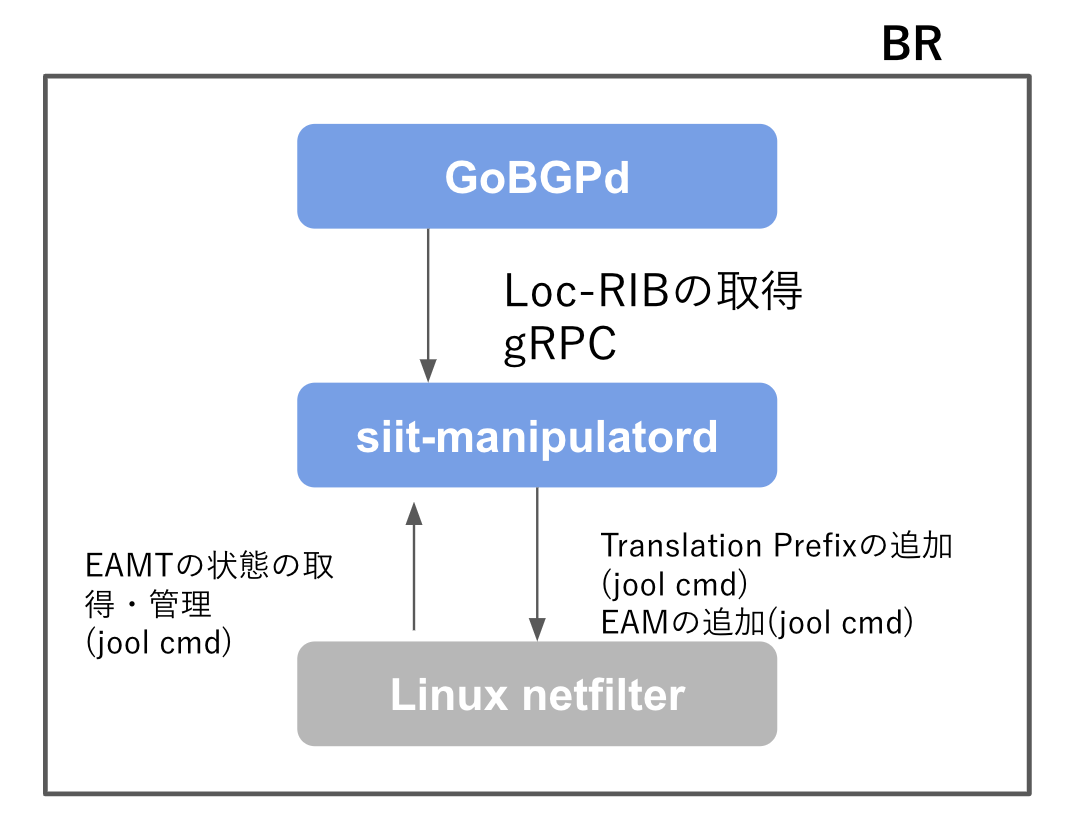
\includegraphics[width=12cm,pagebox=cropbox,clip]{img/poc_implementation.png}
    \end{center}
    \caption{BRに必要なコンポーネント群の関係図}
    \label{fig:poc_implementation}
\end{figure}


\begin{table}[h]
    \label{table:implementation}
    \caption{PoCの実装に利用したソフトウェア群}
    \resizebox{\textwidth}{!}{%
    \begin{tabular}{cllcll}
    \hline
    \multicolumn{2}{c}{ソフトウェア名} & \multicolumn{1}{c}{種別} & \multicolumn{2}{c}{バージョン} & \multicolumn{1}{c}{概要} \\ \hline
    \multicolumn{2}{c}{GoBGP} & BGPデーモン & \multicolumn{2}{c}{2.1.1} & Go言語によって実装されたOSSのBGPデーモン \\ \hline
    \multicolumn{2}{c}{Jool} & SIIT機構 & \multicolumn{2}{c}{4.0.6.2} & SIITやStatefull NAT64をLinux上で動作させるためのOSS. \\ \hline
    \multicolumn{2}{c}{siit-manipulatord} & SIIT制御機構 & \multicolumn{2}{c}{----} & SIIT機構をBGPに伴って制御するための自作アプリケーション \\ \hline
    \multicolumn{2}{c}{Python} & 実行環境 & \multicolumn{2}{c}{3.7.3} & siit-manipulatodに利用する. \\ \hline
    \multicolumn{2}{c}{PyYAML} & ライブラリ & \multicolumn{2}{c}{5.2} & siit-manipulatodに利用.YAML記法で書かれた設定ファイルの読み込みを行う. \\ \hline
    \multicolumn{2}{c}{logzero} & ライブラリ & \multicolumn{2}{c}{1.5.0} & siit-manipulatodに利用.ログファイルの書き出しに利用. \\ \hline
    \end{tabular}%
    }
\end{table}

第\ref{proposal:network:nodes}項で述べたコンポーネント群は以下の様にそれぞれ実装した.
BRにおけるBRに必要なコンポーネント群の関係図を図\ref{fig:poc_implementation}に示す.表\ref{table:implementation}にコンポーネント群の情報の概要を示す.


\subsubsection{BGPデーモン}
BGPデーモンには,OSSのBGPデーモンであるGoBGP\footnote{GoBGP \url{https://osrg.github.io/gobgp/}}を利用する.

GoBGPではgRPC\footnote{gRPC Remote Procedure Calls. \url{https://www.grpc.io/}}を用いた操作機構が実装されており,同期・非同期を問わず他のアプリケーションとの連携が容易に行える.
RouteReflector機構もサポートされているため,本PoCでは全てのノードのBGPデーモンとしてこれを利用する.

\subsubsection{SIIT}
SIITにはJool\footnote{Jool  \url{https://jool.mx/en/index.html}}のSIIT モードを利用する.

JoolはLinuxOSで利用できるNAT64/SIIT環境で,Lunux Netfilterによって実装されており,汎用的に様々なプラットフォームでの利用が可能である\cite{Jool,quintero2016performance}.
EAMTの変更には専用のCLIコマンドを利用する.

\subsubsection{EAMT制御機構}
\label{implementation:poc:siit-manipulatord}
BGP上で受信したLoc-RIBをEAMTに反映するために,EAMT制御機構"siit-manipulatord"を実装した.
gRPCによってGoBGPのLoc-RIBの変化を監視し,JoolのCLIコマンドを利用してLinux NetFilterに変更を反映するほか,Translation Prefixの定義などSIITに必要な情報を管理する.

\subsection{メッセージングと状態遷移}
\label{implementation:poc:sequence}

\begin{figure}[H]
    \begin{center}
    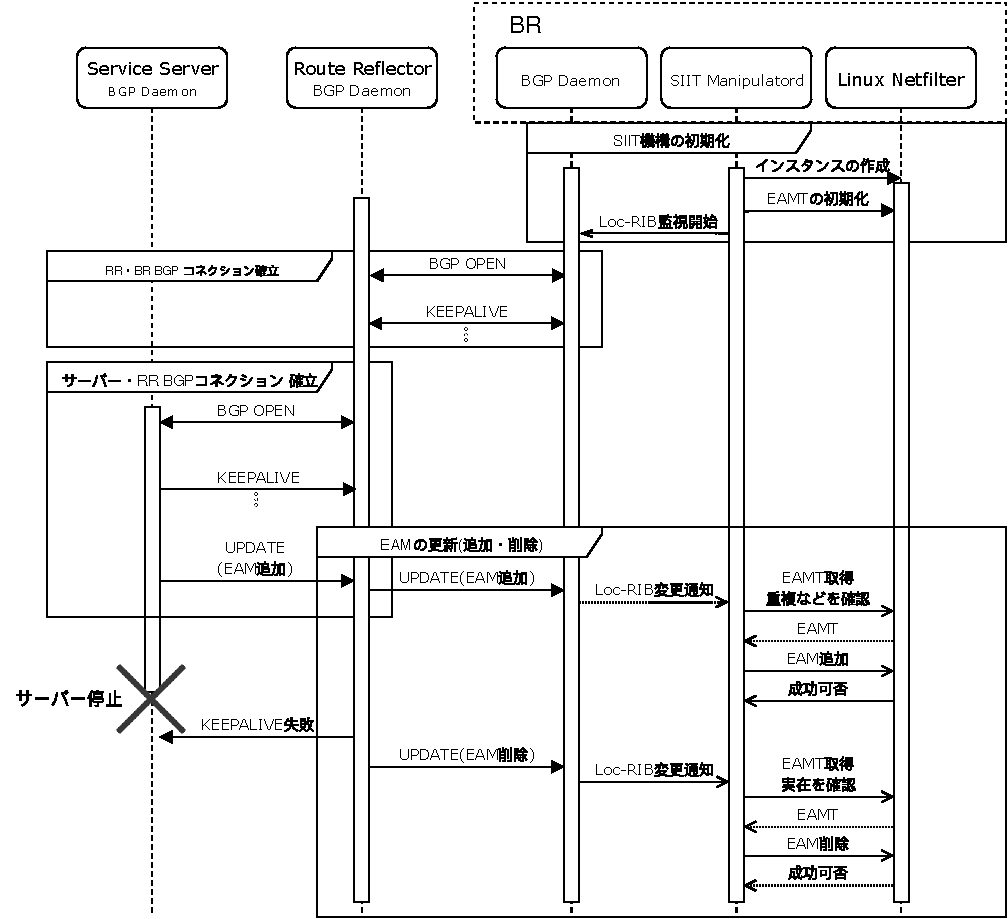
\includegraphics[width=15cm,pagebox=cropbox,clip]{img/sequence_manipulatord.pdf}
    \end{center}
    \caption{本PoCにおける各ホスト・コンポーネントの相互作用と状態遷移}
    \label{fig:poc_implementation}
\end{figure}

図\ref{fig:poc_implementation}にIPv4サービス提供サーバ・ルートリフレクタ・BRの相互作用と状態遷移の概要を示す.

以下に各状態にあるホスト・コンポーネント間の相互作用に関して記述する.

\subsection{SIIT機構の初期化}
BRは起動後ネットワーク環境の準備が出来次第,BGPデーモンとSIIT制御機構のサービスを開始する.EAMT制御機構は初めにLinux Netfilterを操作し,SIITによるプロトコル変換を行う変換インスタンス\footnote{Jool Instance. ネットワーク名前空間ごとに一つ存在可能である.}を作成する.このインスタンスはBRが利用する変換プレフィックスを保持する.その後EAMTを初期化し,gRPCを利用してBGPデーモンからLoc-RIBの監視を開始する.以後Loc-RIBに変更があるまで待機する.Loc-RIBの変更はベストパスの変更に伴っても発生するため,BGP NOTIFICATIONメッセージなどにより,ベストパスとなる経路情報を発信していたBGPピアとのコネクションが切断されたような場合にも,SIIT制御機構に変更通知が送信される.


\subsection{ルートリフレクタ・BR間のBGPコネクションの確立と維持}
BRのBGPデーモンは起動次第,事前に登録されたルートリフレクタに対するBGP OPENメッセージの送信を開始し,BGPコネクションの確立を試みる.
RRからのBGP OPENメッセージの回答を受けてBGPコネクションを確立し,以後BGP KEEPALIVEメッセージによって接続性の死活監視を行う.



\subsection{IPv4サービス提供サーバ・ルートリフレクタ間のBGPコネクションの確立と維持}
IPv4サービス提供サーバのBGPデーモンは起動に伴って,自身のLoc-RIBにEAM(変換プレフィックスとIPv4サービスアドレスによって構成されたNLRIを埋め込んだ経路情報)を登録する.
BGPコネクションが確立次第,IPv4サービス提供サーバはUPDATEメッセージによりEAMの追加をルートリフレクタに通知する.
このコネクションでも同様に,以後BGP KEEPALIVEメッセージによって接続性の死活監視を行う.


\subsection{EAMの追加}
IPv4サービス提供サーバからUPDATEメッセージはルートリフレクタにより各BRに伝達され,UPDATEメッセージを受信したBRのBGPデーモンは自身のLoc-RIBを更新する.

Loc-RIBの更新に伴いLoc-RIBの監視を行っていたSIIT制御機構にgRPCを介し更新通知が送信される.以後のSIIT制御機構の処理はコルーチンを利用した非同期処理によって行われるため,EAMT走査にまつわる処理を行っている最中であってもLoc-RIBの監視はブロッキングされない.

SIIT制御機構はEAMTの更新を滞りなく行うため,LinuxNetfilterに登録された現在のEAMTの状態を取得し,競合するEAMが登録されていないことを確認する.IPv4サービスアドレスとIPv6サービスアドレスが一致するEAMが存在していた場合や事前に登録された変換プレフィックスに一致しない場合,以後の処理をスキップする.

新しく受信したEAMに問題がない場合,SIIT制御機構はEAMの追加を試みる.Linux Nefilterは新しいEAMが追加されたEAMTを参照し,直ちにパケットのフォワーディングを開始する.

\subsection{EAMの削除}
ルートリフレクタは,何らかの理由でIPv4サービス提供サーバとのBGP KEEPALIVEメッセージが失敗した場合やBGP NOTIFICATIONメッセージを受信した場合,自身のLoc-RIBから該当のEAMを削除し,Adj-RIB-OUTの情報を更新する.

ルートリフレクタからEAM削除を広告するBGP UPDATEメッセージを受け取ったBRのBGPデーモンはLoc-RIBを更新し,SIIT制御機構に対してLoc-RIB変更通知を送信する.EAMの追加時と同様に,EAMTを取得して該当するEAMの実在を確認後,SIIT制御機構はEAM削除を試みる.

\subsection{EAMの更新}
BGP経路情報の属性値の変更などに伴ってBRのLoc-RIBに登録されるベストパスが変更になる場合がある.

BRのBGPデーモンはEAM追加・削除時同様に,SIIT制御機構に対してLoc-RIB変更通知を送信する.この変更通知に伴ってEAMT上の古いEAMは削除され,新しいEAMに更新される.




%%% Local Variables:
%%% mode: japanese-latex
%%% TeX-master: "./thesis"
%%% End:
